\documentclass{article}

% Language setting
% Replace `english' with e.g. `spanish' to change the document language
\usepackage[english]{babel}

% Set page size and margins
% Replace `letterpaper' with`a4paper' for UK/EU standard size
\usepackage[a4paper,top=2cm,bottom=2cm,left=3cm,right=3cm,marginparwidth=1.75cm]{geometry}

% Useful packages
\usepackage{amsmath}
\usepackage{graphicx}
\usepackage{listings}
\usepackage{xcolor}
\usepackage[colorlinks=true, allcolors=blue]{hyperref}

\usepackage{algorithm, algpseudocode}
\usepackage{csquotes}
\usepackage{subfig}

\usepackage{parskip} 
\setlength{\parskip}{10pt} 

\definecolor{codegreen}{rgb}{0,0.6,0}
\definecolor{codegray}{rgb}{0.5,0.5,0.5}
\definecolor{codepurple}{rgb}{0.58,0,0.82}
\definecolor{backcolour}{rgb}{0.95,0.95,0.92}

\lstdefinestyle{mystyle}{
    backgroundcolor=\color{backcolour},   
    commentstyle=\color{codegreen},
    keywordstyle=\color{magenta},
    numberstyle=\tiny\color{codegray},
    stringstyle=\color{codepurple},
    basicstyle=\ttfamily\footnotesize,
    breakatwhitespace=false,         
    breaklines=true,                 
    captionpos=b,                    
    keepspaces=true,                 
    numbers=left,                    
    numbersep=5pt,                  
    showspaces=false,                
    showstringspaces=false,
    showtabs=false,                  
    tabsize=2
}

\lstset{style=mystyle}
\newcommand{\code}[1]{\lstinline|#1|}
\setlength\parindent{0pt}

\title{Homework 5\\CS3316 Reinforce learning}
\author{Ng Tze Kean\\Student number: 721370290002}

\begin{document}

\begin{titlepage}
    \begin{center}
        \vfill

        
\includegraphics[width=4cm]{sjtu.png}

        \vspace{1cm}

        \textbf{\huge Shanghai Jiao Tong University}

        \vspace{0.5cm}

        {\large RL C3316 Final Project}

        \vspace{1.5cm}

        Ng Tze Kean\\Student number: 721370290002

    \end{center}
\end{titlepage}

\section*{Introduction}

In this experiment we implement value based RL for Atari and policy based RL
for MuJuCo. In both environments we make use of OpenAI gym environment to
simulate the environment for the agent. In each of the environment,we allow
multiple choices for the user to test the agents on different choice of
environment as stated in the requirements.

\section*{Requirements}

The code can be run as specified. Examples will be provided in this section on
how to use the the program. There will be a need to install all packages before
the code can run. Note the following requirements after installing all prompted
packages:

\begin{itemize}
    \item Python 3.11.19
    \item gymnasium[atari,accept-rom-license]
    \item gymnasium[mujoco]
\end{itemize}

To install the following requirements you can run the script below

\begin{lstlisting}[language=bash]
    pip install "gymnasium[atari,accept-rom-license]"
    pip install "gymnasium[mujoco]"
\end{lstlisting}

\section*{Usage}

For Atari experiment specify the first argument as \code{atari} with the
following optional arguments. The environments that will work in this setup are
the following [VideoPinball-ramNoFrameskip-v4, BreakoutNoFrameskip-v4,
        PongNoFrameskip-v4, BoxingNoFrameskip-v4] and the dueling argument is a boolean
specifier. Do note that you have to specify the argument as a capitalized
option.

\begin{lstlisting}[language=bash]
python3.11 run.py --exp atari --env_name ENV --is_dueling BOOL
\end{lstlisting}

For Mujoco, the following arguments can also be specified. That is, only the
first option is required. Note that for the environments that can be specified,
the following environments can be tested on: [Hopper-v4, Humanoid-v4,
HalfCheetah-v4, Ant-v4] and the method option allows the user to choose between
    [PPO, SAC] as the agent of choice.

\begin{lstlisting}[language=bash]
python3.11 run.py --exp mujoco --env_name ENV --method METHOD
\end{lstlisting}

\newpage

\section*{Implementation}

The implementation of the code is as follows. The code is split into two main
files, namely \code{atari.py} and \code{mujoco.py}. The code is then imported
into the main file \code{run.py} to run the experiment. In both experiments we
make use of the OpenAI gym environment to simulate the environment for the
agent.

\subsection*{Atari}

The Atari environment consists of classic video games like Pong, Breakout, and
Space Invaders. Unlike MuJoCo's focus on physics simulation, Atari environments
provide a high-dimensional visual input space with discrete action sets (e.g.,
up, down, jump, fire). The agent interacts with the game through its actions
and observes the screen as its primary source of information. Rewards are
typically sparse, meaning they are only received for achieving specific goals
(e.g., points in a game).

In the atari experiment, we implement a value based RL agent. The agent
designed are the DQN and Dueling DQN.

\subsubsection*{Value based agent}

\textbf{DQN (Deep Q-Network)}: DQN is a deep learning-based off-policy algorithm that
utilizes a neural network to approximate the Q-value function. This function
estimates the expected future reward for taking a specific action in a given
state. The agent interacts with the Atari environment, observes the screen, and
takes an action. Based on the reward received and the next observed state, the
Q-network is updated to improve its estimation of future rewards.

The key components of DQN include:

\begin{enumerate}
    \item Q-Network: A neural network that approximates the Q-value function. It takes
          the state as input and outputs Q-values for all possible actions.
    \item Target Network: A copy of the Q-network, used to compute target Q-values. It is
          updated periodically to stabilize training.
    \item Experience Replay: A buffer that stores past experiences (state, action,
          reward, next state). Mini-batches are sampled from this buffer to break the
          correlation between consecutive experiences.
\end{enumerate}

Training process:

\begin{enumerate}
    \item Initialization: Initialize the Q-network with random weights. Create a copy of
          the Q-network as the target network.
    \item Interaction: The agent interacts with the environment, observing states and
          taking actions based on an epsilon-greedy policy (choosing random actions with
          probability $\epsilon$ and greedy actions with probability $1-\epsilon$)
    \item Experience Storage: Store the experiences (state, action, reward, next state)
          in the replay buffer.
    \item Mini-Batch Sampling: Randomly sample a mini-batch of experiences from the
          replay buffer.
    \item Q-Value Update: Update the Q-values using the Bellman equation
    \item Target Network Update: Periodically update the target network with the
          Q-network weights.
\end{enumerate}

\textbf{DDQN (Double DQN)}: DDQN is an improvement over DQN that addresses the
overestimation issue sometimes encountered with DQN. It introduces separate
networks for estimating the Q-value (evaluation network) and selecting the
action (target network). This separation reduces the overestimation bias and
can lead to more stable learning. The overall training process is similar in
nature to DQN as explained above and we will examine the advantage of
separating the network for estimating the Q-value. The class for DDQN can also
be examined under the code base in the class \code{dueling_DQN}.

\subsubsection*{Set up}

The agent is then trained on the environment specified by the \code{env_name}
argument. The agent is then trained for a number of episodes which is currently
fixed at 8000000 as we have found that the agent is likely to converge at when
the number of episodes is around 8000000.

As the agent is being trained, we evaluate per some fixed number of episodes to
see how well the agent is performing. The evaluation is done by running the
agent on the environment without updating the weights of the agent. We log the
performance of the agent in a csv file which can then be used to plot the
performance of the agent.

Since there are are a variety of atari games, we allow the user to specify the
atari game that they want to train the agent on. For this experiment, we have
trained the agent over different environments listed in the requirements and we
compare the performance of the agent on each of the environment. Some of the
environments trained on include Breakout and Pong which we will use to analyse
the performance of the agent.

\subsection*{MuJoCo}

MuJoCo is a physics engine specifically designed for simulating physical
systems commonly encountered in robotics. It provides a rich set of
environments for reinforcement learning tasks, often involving legged
locomotion or manipulation. These environments typically involve a simulated
character interacting with the environment, receiving rewards based on its
actions and achieving specific goals (e.g., walking forward for a certain
distance).

In the mujoco experiment, we implement a policy based RL agent. The agent
designed are the SAC and PPO.

\subsubsection*{Policy based agent}

\textbf{Soft Actor-Critic (SAC)}: SAC is an off-policy algorithm that combines elements
of Deep Deterministic Policy Gradients (DDPG) and maximum entropy policies. It
learns a policy that maximizes expected return while also encouraging
exploration. The agent interacts with the environment, taking actions and
receiving rewards. This information is used to update both the policy and a
value function that estimates the expected future return. The entropy bonus
term in the objective function promotes diverse exploration, potentially
leading to better performance in the long run.

Training process:

\begin{enumerate}
    \item Initialization: Initialize the policy network, Q-networks, and the target
          Q-networks with random weights.
    \item Interaction: The agent interacts with the environment, collecting transitions
          of states, actions, rewards, and next states.
    \item Experience Storage: Store the transitions in a replay buffer.
    \item Q-Value Update: Sample mini-batches from the replay buffer and update the
          Q-networks by minimizing the mean squared error loss.
    \item Policy Update: Update the policy network by minimizing the entropy-augmented
          objective.
    \item Target Network Update: Periodically update the target Q-networks to slowly
          track the Q-networks.
    \item Repeat: Continue the process until convergence.
\end{enumerate}

Overall, SAC leverages entropy maximization to balance exploration and
exploitation, ensuring robust learning. The use of twin Q-networks reduces
overestimation bias, leading to more accurate value estimates and improved
policy performance.

\textbf{Proximal Policy Optimization (PPO)}: PPO is an on-policy algorithm that focuses
on maintaining a policy close to the one used for collecting data during
training. This is achieved by clipping the policy update during training to
ensure it remains similar to the original policy. PPO interacts with the
environment, collects data, and then updates the policy to improve its
performance while maintaining stability by keeping the updates within a certain
range.

\begin{enumerate}
\item Clipped Surrogate Objective
PPO uses a clipped objective function to restrict the change in policy:
\[
    L^{CLIP}(\theta) = E_t \left[ \min \left( r_t(\theta) \hat{A}_t, \text{clip}(r_t(\theta), 1 - \epsilon, 1 + \epsilon) \hat{A}_t \right) \right]
\]
where \( r_t(\theta) \) is the probability ratio between the new and old
policies, \( \hat{A}_t \) is the estimated advantage, and \( \epsilon \) is a
hyperparameter controlling the clipping range.


\item Advantage Estimation
PPO uses Generalized Advantage Estimation (GAE) to compute the advantage
function, providing a trade-off between bias and variance:
\[
    \hat{A}_t = \sum_{l=0}^{\infty} (\gamma \lambda)^l \delta_{t+l}
\]
where \( \delta_t = r_t + \gamma V(s_{t+1}) - V(s_t) \), and \( \lambda \) is
the GAE parameter.

\end{enumerate}

Training Process:

\begin{enumerate}
    \item Initialization: Initialize the policy and value networks with random weights.
    \item Interaction: The agent interacts with the environment, collecting trajectories of states, actions, rewards, and next states.
    \item Advantage Calculation: Compute the advantage estimates using GAE.
    \item Policy Update: Update the policy network by optimizing the clipped surrogate objective using gradient ascent.
    \item Value Update: Update the value network by minimizing the mean squared error between the predicted and actual returns.
    \item Repeat: Continue the process until convergence.
\end{enumerate}

PPO optimizes a surrogate objective that balances exploration and exploitation,
ensuring stable updates to the policy. The clipping mechanism prevents large
deviations in policy updates, leading to more reliable and efficient learning.

We also train the agent on a variety of environments in the mujoco environment.
Some of the environments trained on include HalfCheetah and Hopper which we
will analyze the agent on in the next section.

\newpage

\section*{Results}

\subsection*{Atari}

Both DQN and DDQN agents learn through trial and error by interacting with the
Atari games. They process the screen images as input and predict the Q-values
for each possible action. The agent then selects the action with the highest
predicted Q-value (greedy action selection) or explores alternative options
with a certain probability (exploration strategy). As the agent receives
rewards and experiences new states, it updates its Q-network to improve its
understanding of the environment and the value of different actions within each
state.

\begin{figure}[h]
    \centering
    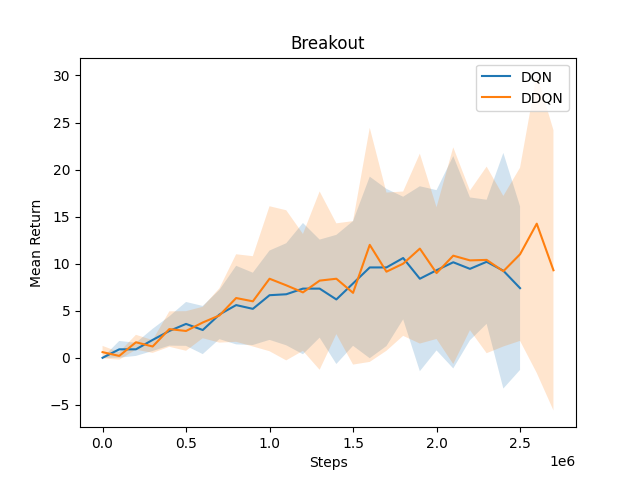
\includegraphics[width=0.5\textwidth]{img/breakout.png}
    \caption{Performance DQN and DDQN on Atari Breakout}
\end{figure}

As you can see from the graph above that the agent is has not been able to
learn from the environment given the number of episodes. As we are training the
agent on a personal laptop with limited computational power, we are unable to
train the agent sufficiently fast enough such that it converges. Hence, for the
evaluation of the agent, we will refer to online sources that have achieved
results for comparison. We look to github to search for graphs and we find that
that the number of episodes needed ranges in the value of 20million to
50million episodes which we are not able to achieve. Currently to reach
5million episodes, my personal laptop has to run for over 2 days. We now
proceed to perform the comparison of these 2 agents over Breakout and Pong
environment.

Learning Speed and Convergence: DDQN generally exhibits faster and more stable
convergence compared to DQN. This is because DDQN mitigates the overestimation
bias in Q-value estimation, leading to more accurate learning.

Algorithm Stability: DDQN is considered more stable than DQN due to the
decoupling of the evaluation and target networks. This reduces the compounding
effect of overestimation errors in DQN, leading to smoother learning in DDQN.

Training Time and Efficiency: Due to its improved stability and learning speed,
DDQN can achieve good performance in less training time compared to DQN. While
DQN might require extensive training to overcome overestimation issues, DDQN
can reach convergence faster with potentially less computational resources
needed.

\subsection*{Mujoco}

Unlike the case of Atari which we are not able to achieve

\begin{figure}[h]
    \centering
    \subfloat[Ant]{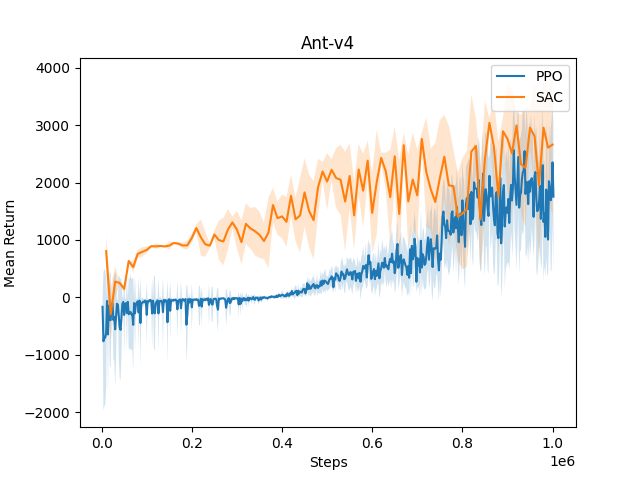
\includegraphics[width=0.5\textwidth]{img/ant.png}}
    \subfloat[Half Cheetah]{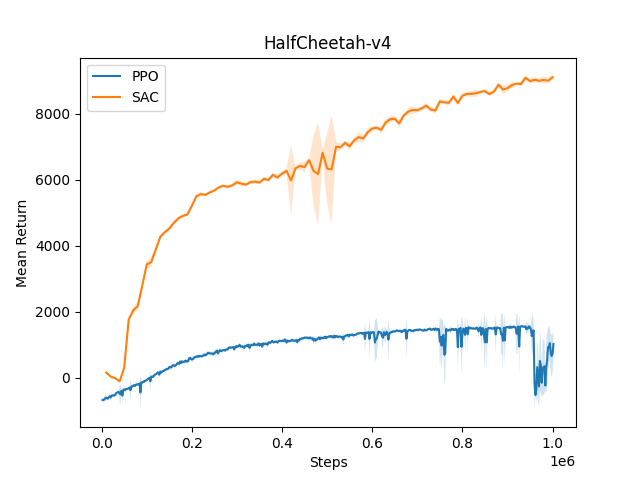
\includegraphics[width=0.5\textwidth]{img/half_cheetah.png}}
    \caption{Performance SAC and PPO on Mujoco environment}
\end{figure}

Learning Speed and Convergence: SAC often exhibits faster initial learning
compared to PPO. This is because SAC's entropy bonus encourages exploration,
allowing it to discover effective strategies quicker. However, PPO's focus on
policy stability ensures smoother convergence in the later stages of training.

Algorithm Stability: PPO is generally considered more stable than SAC. PPO's
clipped objective function prevents drastic policy changes, reducing the risk
of the agent diverging from good policies during training. SAC, while effective
at exploration, can sometimes lead to unstable learning behavior if
hyperparameters are not carefully tuned.

Training Time and Efficiency: Due to its faster initial learning, SAC might
achieve good performance in less training time compared to PPO. However, PPO's
stability can lead to more efficient training in the long run, as it avoids the
need for extensive hyperparameter tuning to prevent divergence.

\begin{figure}[h]
    \centering
    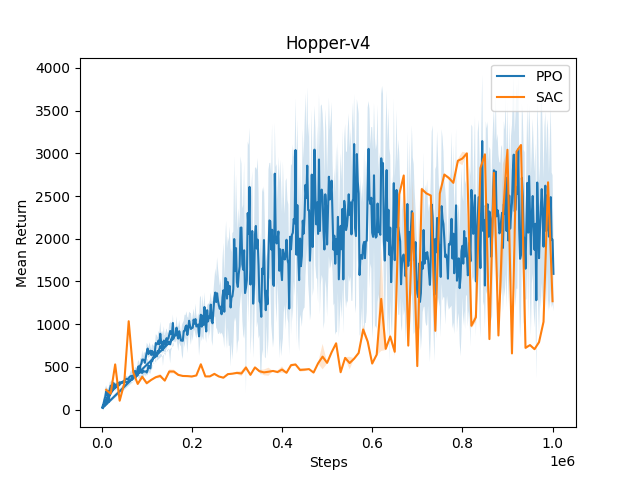
\includegraphics[width=0.5\textwidth]{img/hopper.png}
    \caption{Performance SAC and PPO on Mujoco Hopper}
\end{figure}

Although, it is interesting to note that in the case of Hopper, the PPO agent
is able to perform better than the SAC agent. This is likely due to the nature
of the environment and the characteristics of the algorithms. The Hopper
environment may benefit from PPO's stability and policy consistency, leading to
better performance compared to SAC.

\end{document}